%!TEX program = xelatex
%# -*- coding: utf-8 -*-
%!TEX encoding = UTF-8 Unicode

\documentclass[12pt,oneside,a4paper]{article}\usepackage[]{graphicx}\usepackage[]{xcolor}
%% maxwidth is the original width if it is less than linewidth
%% otherwise use linewidth (to make sure the graphics do not exceed the margin)
\makeatletter
\def\maxwidth{ %
  \ifdim\Gin@nat@width>\linewidth
    \linewidth
  \else
    \Gin@nat@width
  \fi
}
\makeatother

\definecolor{fgcolor}{rgb}{0, 0, 0}
\newcommand{\hlnum}[1]{\textcolor[rgb]{0,0,0}{#1}}%
\newcommand{\hlstr}[1]{\textcolor[rgb]{0,0,1}{#1}}%
\newcommand{\hlcom}[1]{\textcolor[rgb]{0.443,0.478,0.702}{#1}}%
\newcommand{\hlopt}[1]{\textcolor[rgb]{0,0,0}{#1}}%
\newcommand{\hlstd}[1]{\textcolor[rgb]{0,0,0}{#1}}%
\newcommand{\hlkwa}[1]{\textcolor[rgb]{0.498,0,0.333}{\textbf{#1}}}%
\newcommand{\hlkwb}[1]{\textcolor[rgb]{0.498,0,0.333}{\textbf{#1}}}%
\newcommand{\hlkwc}[1]{\textcolor[rgb]{0.498,0,0.333}{\textbf{#1}}}%
\newcommand{\hlkwd}[1]{\textcolor[rgb]{0,0,0}{#1}}%

\usepackage{framed}
\makeatletter
\newenvironment{kframe}{%
 \def\at@end@of@kframe{}%
 \ifinner\ifhmode%
  \def\at@end@of@kframe{\end{minipage}}%
  \begin{minipage}{\columnwidth}%
 \fi\fi%
 \def\FrameCommand##1{\hskip\@totalleftmargin \hskip-\fboxsep
 \colorbox{shadecolor}{##1}\hskip-\fboxsep
     % There is no \\@totalrightmargin, so:
     \hskip-\linewidth \hskip-\@totalleftmargin \hskip\columnwidth}%
 \MakeFramed {\advance\hsize-\width
   \@totalleftmargin\z@ \linewidth\hsize
   \@setminipage}}%
 {\par\unskip\endMakeFramed%
 \at@end@of@kframe}
\makeatother

\definecolor{shadecolor}{rgb}{.97, .97, .97}
\definecolor{messagecolor}{rgb}{0, 0, 0}
\definecolor{warningcolor}{rgb}{1, 0, 1}
\definecolor{errorcolor}{rgb}{1, 0, 0}
\newenvironment{knitrout}{}{} % an empty environment to be redefined in TeX

\usepackage{alltt}
\usepackage{geometry}
\geometry{verbose,tmargin=2cm,bmargin=2cm,lmargin=2cm,rmargin=2cm}
\usepackage[pdfusetitle,
 bookmarks=true,bookmarksnumbered=true,bookmarksopen=true,bookmarksopenlevel=2,
 breaklinks=false,pdfborder={0 0 1},backref=false,colorlinks=false]
 {hyperref}
\hypersetup{pdfstartview={XYZ null null 1}}
\usepackage{url}
\setcounter{secnumdepth}{2}
\setcounter{tocdepth}{2}
\usepackage{microtype}

\usepackage{amsmath, amsthm, amssymb, amsfonts}
\usepackage[retainorgcmds]{IEEEtrantools}

\usepackage{algorithm}
\usepackage{algorithmic}
\renewcommand{\algorithmicrequire}{\textbf{Input:}} 
\renewcommand{\algorithmicensure}{\textbf{Output:}} 

\usepackage[sc]{mathpazo}
\linespread{1.1}
\usepackage[T1]{fontenc}


\usepackage{graphics}
\usepackage{graphicx}
\usepackage[figure]{hypcap}
\usepackage[hypcap]{caption}
\usepackage{tikz}
%\usepackage{grffile} 
%\usepackage{float} 
\usepackage{pdfpages}

\usepackage{multirow}
\usepackage{booktabs}
\usepackage{threeparttable}

%\usepackage[square,numbers,super,comma,sort]{natbib}
%\usepackage[backend=biber, style=nature, sorting=none, isbn=false, url=false, doi=false]{biblatex}
%\addbibresource{ref.bib}
%\usepackage[]{authblk}

\usepackage{verbatim}

\newcommand{\problem}[1]
{
    \clearpage
    \section*{Problem {#1}}
}

\newcommand{\subproblem}[1]
{
    \subsection*{Problem {#1}}
}


\newcommand{\solution}
{
    \vspace{15pt}
    \noindent\ignorespaces\textbf{\large Solution}\par
}

\usepackage{fancyhdr}
\usepackage{extramarks}
\lhead{\hmwkAuthorName}
\chead{\hmwkTitle}
\rhead{\firstxmark}
\cfoot{\thepage}

\newcommand{\hmwkTitle}{STAT 8051 HW 4}
\newcommand{\hmwkAuthorName}{Jingxiang Li}

\setlength\headheight{15pt}
\setlength\parindent{0pt}
\setlength{\parskip}{0.5em}

\newcommand{\m}[1]{\texttt{{#1}}}


\pagestyle{fancy}

\title{\hmwkTitle}
\author{\hmwkAuthorName}
\date{\today}
\IfFileExists{upquote.sty}{\usepackage{upquote}}{}
\begin{document}

\maketitle



\problem{7.8}
Sue fits a wls regression with all weights equal to 2. Joe fits a wls regression to the same data with all weights equal to 1. What are the differences in estimates of coefficients, standard errors, $\sigma^{2}$ F-tests between Sue’s and Joe’s analyses?

\solution
Let \m{m1} be the regression model fitted by Sue with weights all equal to 2; \m{m2} be the regression model fitted by Joe, where all weights equal to 1. Since they both use constant weights, the estimates of coefficients and the F-tests should be the same, but the standard errors and $\sigma^{2}$ are different between these two models, but it's only a scale difference.

Claim that $W_{1}$ and $W_{2}$ are the weighting matrix respectively for \m{m1} and \m{m2}, so that we have $W_{1} = 2I$, $W_{2} = I$, where $I$ is the $n\times n$ identity matrix. For the coefficient estimator, we have 
$$\hat{\beta} = (X'WX)^{-1}X'WY$$
Let $\hat{\beta}_{1}$ be the estimator obtained from \m{m1}, $\hat{\beta}_{2}$ be the estimator obtained from \m{m2}, so that 
$$\hat{\beta}_{1} = (X' \times 2I \times X)^{-1}X'\times 2I \times Y = (X'X)^{-1}X'Y = \hat{\beta}_{2}$$
so that the estimates of coefficients between two models are the same.

Let $e_{i}$ be the residual vectors from model \m{mi}, $RSS_{i}$ be the $RSS$ derived from model \m{mi}, $\sigma^{2}_{i}$ be the $\sigma^{2}$ from model \m{mi}, where $i = 1,2$. and let $df$ be the degree of freedom. we have
$$RSS_{1} = e_{1}'W_{1}e_{1} = 2e_{1}'e_{1}$$
$$RSS_{2} = e_{2}'W_{2}e_{2} = e_{1}'e_{1}$$
Note that the estimates of coefficients between two models are the same, so that $e_{1} = e_{2}$, and $RSS_{1} = 2RSS_{2}$, and
$$\hat{\sigma}_{1}^{2} = \frac{RSS_{1}}{df} = \frac{2RSS_{2}}{df} = 2\hat{\sigma}_{2}^{2}$$
then we have
$$\hat{\sigma}_{1} = \sqrt{2}\hat{\sigma}_{2}$$

For $\sigma^{2}$, based on the error assumption of WLS, we have $Var(e_{1i}) = \sigma_{1}^{2} / 2$, $Var(e_{2i}) = \sigma_{2}^{2}$, and note that $e_{1i} = e_{2i}, \forall i$, so that $$\sigma_{1}^{2} = 2\sigma_{2}^{2}$$

Let $F_{i}$ be the $F$ statistic for model \m{mi}, where $i=1,2$, and let $n$ be the sample size.
$$\begin{aligned}
F_{1} &= \frac{(\sum{2(y_{i} - \bar{y})^2} - RSS_{1}) / (n - 1 - df)}{RSS_{1}/df}\\
F_{1} &= \frac{(\sum{2(y_{i} - \bar{y})^2} - 2RSS_{2}) / (n - 1 - df)}{2RSS_{2}/df}\\
F_{1} &= \frac{(\sum{(y_{i} - \bar{y})^2} - RSS_{2}) / (n - 1 - df)}{RSS_{2}/df}\\
F_{1} &= F_{2}
\end{aligned}$$

In summary, we have
$$\hat{\beta}_{1} = \hat{\beta}_{2}$$
$$\hat{\sigma}_{1} = \sqrt{2}\hat{\sigma}_{2}$$
$$\sigma_{1}^{2} = 2\sigma_{2}^{2}$$
$$F_{1} = F_{2}$$
Q.E.D.

\problem{7.7}
\textbf{Galton’s sweet peas} (Data file: \m{galtonpeas}) Many of the ideas of regression first appeared in the work of Sir Francis Galton (1822–1911) on the inheritance of characteristics from one generation to the next. In Galton (1877), he discussed experiments on sweet peas. By comparing the sweet peas produced by parent plants to those produced by offspring plants, he could observe inheritance from one generation to the next. Galton categorized parent plants according to the typical diameter of the peas they produced. For seven size classes from 0.15 to 0.21 inches, he arranged for each of nine of his friends to grow 10 plants from seed in each size class; however, two of the crops were total failures. A summary of Galton’s data were later published in Pearson (1930). The data file includes \m{Parent} diameter, \m{Progeny} diameter, and \m{SD} the standard deviation of the progeny diameters. Sample sizes are unknown but are probably large.

\subproblem{7.7.1}
Draw the scatterplot of \m{Progeny} versus \m{Parent}.

\solution
\begin{knitrout}
\definecolor{shadecolor}{rgb}{1, 1, 1}\color{fgcolor}\begin{kframe}
\begin{alltt}
\hlkwd{require}\hlstd{(alr4)}
\hlkwd{require}\hlstd{(ggplot2)}
\hlstd{data} \hlkwb{<-} \hlstd{galtonpeas}
\hlstd{p} \hlkwb{<-} \hlkwd{ggplot}\hlstd{(}\hlkwc{data} \hlstd{= data,} \hlkwd{aes}\hlstd{(}\hlkwc{x} \hlstd{= Parent,} \hlkwc{y} \hlstd{= Progeny))}
\hlstd{p} \hlkwb{<-} \hlstd{p} \hlopt{+} \hlkwd{geom_point}\hlstd{()}
\hlstd{p} \hlkwb{<-} \hlstd{p} \hlopt{+} \hlkwd{theme_bw}\hlstd{()} \hlopt{+} \hlkwd{theme}\hlstd{(}\hlkwc{text} \hlstd{=} \hlkwd{element_text}\hlstd{(}\hlkwc{size} \hlstd{=} \hlnum{12}\hlstd{))}
\hlstd{p} \hlkwb{<-} \hlstd{p} \hlopt{+} \hlkwd{ggtitle}\hlstd{(}\hlstr{"Progeny VS Parent"}\hlstd{)}
\hlstd{p}
\end{alltt}
\end{kframe}

{\centering 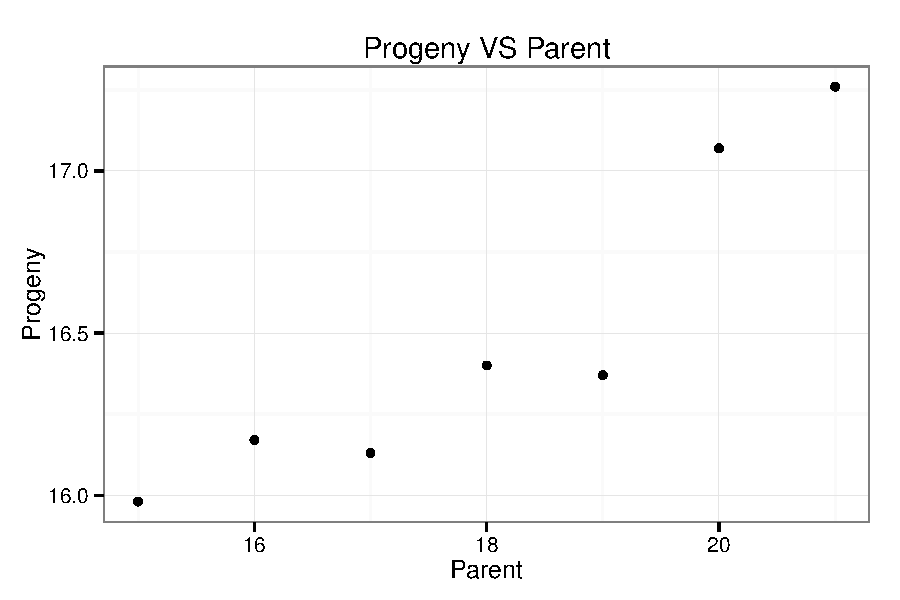
\includegraphics[width=.8\linewidth]{figure/p771} 

}



\end{knitrout}

\subproblem{7.7.2}
Assuming that the standard deviations given are population values, compute the weighted regression of \m{Progeny} on \m{Parent}. Draw the fitted mean function on your scatterplot.

\solution
\begin{knitrout}
\definecolor{shadecolor}{rgb}{1, 1, 1}\color{fgcolor}\begin{kframe}
\begin{alltt}
\hlstd{model} \hlkwb{<-} \hlkwd{lm}\hlstd{(Progeny} \hlopt{~} \hlstd{Parent,} \hlkwc{data} \hlstd{= data,} \hlkwc{weights} \hlstd{=} \hlnum{1} \hlopt{/} \hlstd{data}\hlopt{$}\hlstd{SD}\hlopt{^}\hlnum{2}\hlstd{)}
\hlstd{coef} \hlkwb{<-} \hlstd{model}\hlopt{$}\hlstd{coefficients}

\hlstd{p} \hlkwb{<-} \hlstd{p} \hlopt{+} \hlkwd{geom_abline}\hlstd{(}\hlkwc{intercept} \hlstd{= coef[}\hlnum{1}\hlstd{],} \hlkwc{slope} \hlstd{= coef[}\hlnum{2}\hlstd{])}
\hlstd{p}
\end{alltt}
\end{kframe}

{\centering 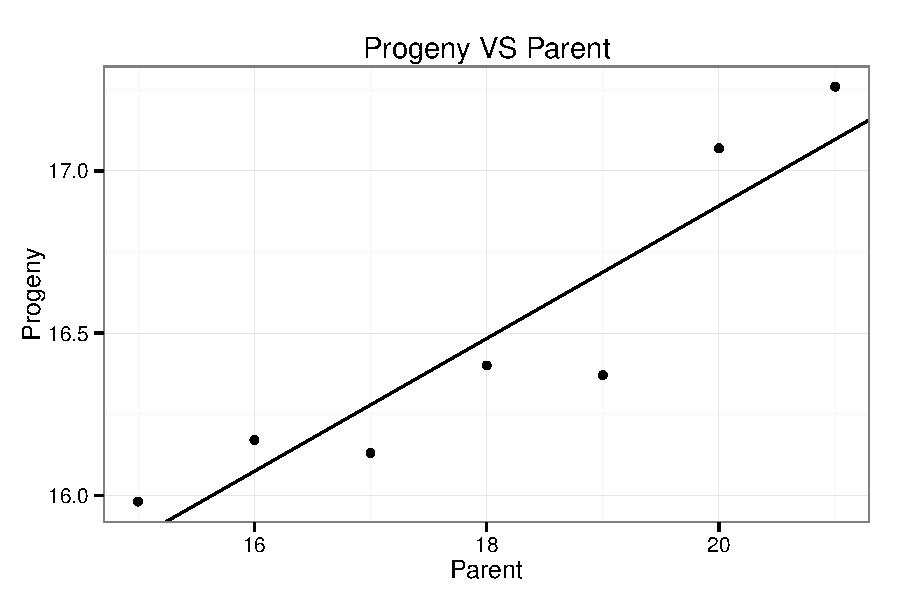
\includegraphics[width=.8\linewidth]{figure/p772} 

}



\end{knitrout}

\subproblem{7.7.3}
Galton took the average size of all peas produced by a plant to determine the size class of the parental plant. Yet for seeds to represent that plant and produce offspring, Galton chose seeds that were as close to the overall average size as possible. Thus, for a small plant, the exceptional large seed was chosen as a representative, while larger, more robust plants were represented by relatively smaller seeds. What effects would you expect these experimental biases to have on (1) estimation of the intercept and slope and (2) estimates of error?

\solution
Following the way Galton determine the seeds that represent the parent plant, the estimation of the slope will be lower than the true nature, and thus the intercept term will increase, and the variance will increase too. 

Due to the fact that larger seeds are chosen for small plant, smaller seeds are chosen for large plant, the offspring's size will be centralized. It means that for each level of \m{Parent}, \m{Progeny} are more closer to each other compared with the true nature, so that the slope coefficient will decrease. Then, since the central point for this regression model won't change too much and the slope will decrease, the intercept will increase. Then for the variance of model, since Galton choose exceptional large or small seeds to represent parent plant, the variance of \m{Progeny}'s size for each level of \m{Parent} will definitely increase. 

\problem{7.8}
\textbf{Jevons’s gold coins} (Data file: \m{jevons}) The data in this example are deduced from a diagram in Jevons (1868) and provided by Stephen M. Stigler. In a study of coinage, Jevons weighed 274 gold sovereigns that he had collected from circulation in Manchester, England. For each coin, he recorded the weight after cleaning to the nearest 0.001 g, and the date of issue. The data file includes \m{Age}, the age of the coin in decades, \m{n}, the number of coins in the age class, \m{Weight}, the average weight of the coins in the age class, \m{SD}, the standard deviation of the weights. The minimum \m{Min} and maximum \m{Max} of the weights are also given. The standard weight of a gold sovereign was 7.9876 g; the minimum legal weight was 7.9379 g.

\subproblem{7.8.1}
Draw a scatterplot of \m{Weight} versus \m{Age}, and comment on the applicability of the usual assumptions of the linear regression model. Also draw a scatterplot of \m{SD} versus \m{Age}, and summarize the information in this plot.

\solution
\begin{knitrout}
\definecolor{shadecolor}{rgb}{1, 1, 1}\color{fgcolor}\begin{kframe}
\begin{alltt}
\hlkwd{require}\hlstd{(gridExtra)}
\hlstd{data} \hlkwb{<-} \hlstd{jevons}

\hlstd{p1} \hlkwb{<-} \hlkwd{ggplot}\hlstd{(}\hlkwc{data} \hlstd{= data,} \hlkwd{aes}\hlstd{(}\hlkwc{x} \hlstd{= Age,} \hlkwc{y} \hlstd{= Weight))}
\hlstd{p1} \hlkwb{<-} \hlstd{p1} \hlopt{+} \hlkwd{geom_point}\hlstd{()}
\hlstd{p1} \hlkwb{<-} \hlstd{p1} \hlopt{+} \hlkwd{geom_smooth}\hlstd{(}\hlkwc{formula} \hlstd{= y} \hlopt{~} \hlstd{x,} \hlkwc{method} \hlstd{=} \hlstr{"lm"}\hlstd{,} \hlkwc{se} \hlstd{=} \hlnum{FALSE}\hlstd{)}
\hlstd{p1} \hlkwb{<-} \hlstd{p1} \hlopt{+} \hlkwd{theme_bw}\hlstd{()} \hlopt{+} \hlkwd{theme}\hlstd{(}\hlkwc{text} \hlstd{=} \hlkwd{element_text}\hlstd{(}\hlkwc{size} \hlstd{=} \hlnum{14}\hlstd{))}
\hlstd{p1} \hlkwb{<-} \hlstd{p1} \hlopt{+} \hlkwd{ggtitle}\hlstd{(}\hlstr{"Weight VS Age"}\hlstd{)}

\hlstd{p2} \hlkwb{<-} \hlkwd{ggplot}\hlstd{(}\hlkwc{data} \hlstd{= data,} \hlkwd{aes}\hlstd{(}\hlkwc{x} \hlstd{= Age,} \hlkwc{y} \hlstd{= SD))}
\hlstd{p2} \hlkwb{<-} \hlstd{p2} \hlopt{+} \hlkwd{geom_point}\hlstd{()}
\hlstd{p2} \hlkwb{<-} \hlstd{p2} \hlopt{+} \hlkwd{geom_smooth}\hlstd{(}\hlkwc{formula} \hlstd{= y} \hlopt{~} \hlstd{x,} \hlkwc{method} \hlstd{=} \hlstr{"lm"}\hlstd{,} \hlkwc{se} \hlstd{=} \hlnum{FALSE}\hlstd{)}
\hlstd{p2} \hlkwb{<-} \hlstd{p2} \hlopt{+} \hlkwd{theme_bw}\hlstd{()} \hlopt{+} \hlkwd{theme}\hlstd{(}\hlkwc{text} \hlstd{=} \hlkwd{element_text}\hlstd{(}\hlkwc{size} \hlstd{=} \hlnum{14}\hlstd{))}
\hlstd{p2} \hlkwb{<-} \hlstd{p2} \hlopt{+} \hlkwd{ggtitle}\hlstd{(}\hlstr{"SD VS Age"}\hlstd{)}

\hlkwd{grid.arrange}\hlstd{(p1, p2,} \hlkwc{ncol}\hlstd{=}\hlnum{2}\hlstd{)}
\end{alltt}
\end{kframe}

{\centering 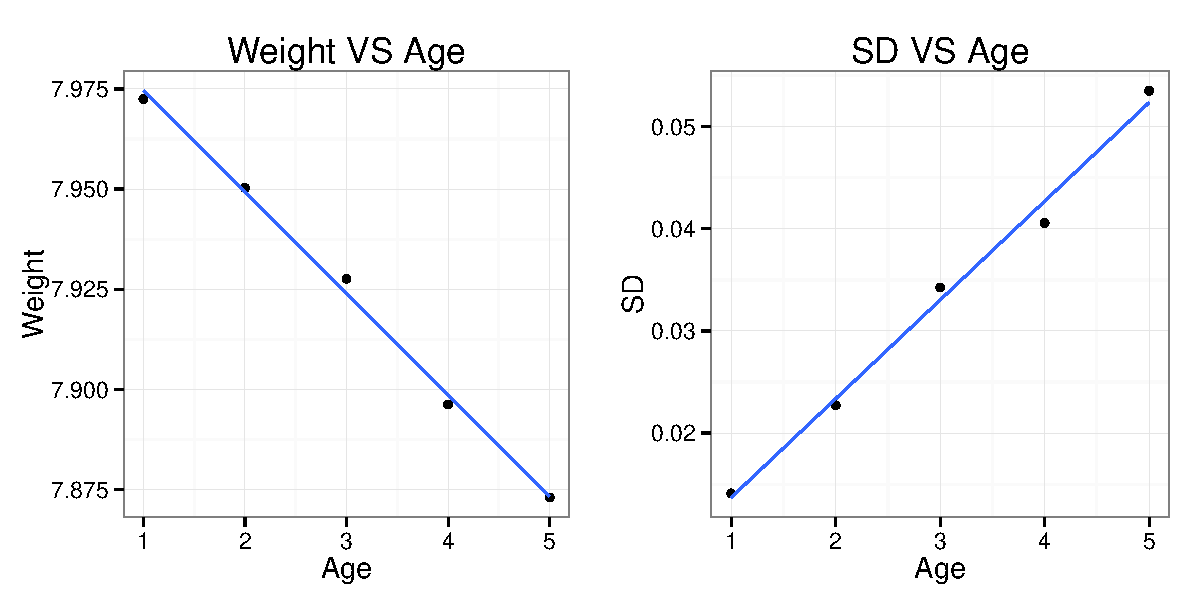
\includegraphics[width=.9\linewidth]{figure/p781} 

}



\end{knitrout}

For the regression model \m{Weight} versus \m{Age}, following the information provided by the scatterplot, the linear form is appropriate and there is no specific information shows that the variance of each case in this dataset is different. However, as the standard deviation for each point is given, we should consider WLS as our primary choice.

For the \m{SD} versus \m{Age} scatterplot, we can see that as \m{Age} goes on, the standard deviation of the weights increase linearly against \m{Age}.

\subproblem{7.8.2}
To fit a simple linear regression model with Weight as the response, wls should be used with variance function $Var(\m{Weight}|\m{Age}) =  \m{n}\sigma^{2}/\m{SD}^{2}$. Sample sizes are large enough to assume the \m{SD} are population values. Fit the wls model.

\solution
\begin{knitrout}
\definecolor{shadecolor}{rgb}{1, 1, 1}\color{fgcolor}\begin{kframe}
\begin{alltt}
\hlstd{w} \hlkwb{<-} \hlstd{data}\hlopt{$}\hlstd{SD}\hlopt{^}\hlnum{2} \hlopt{/} \hlstd{data}\hlopt{$}\hlstd{n}
\hlstd{m} \hlkwb{<-} \hlkwd{lm}\hlstd{(Weight} \hlopt{~} \hlstd{Age,} \hlkwc{data} \hlstd{= data,} \hlkwc{weight} \hlstd{= w)}
\hlkwd{summary}\hlstd{(m)}
\end{alltt}
\begin{verbatim}
## 
## Call:
## lm(formula = Weight ~ Age, data = data, weights = w)
## 
## Weighted Residuals:
##         1         2         3         4         5 
## -5.21e-06 -5.23e-07  1.94e-05 -2.07e-05  8.66e-06 
## 
## Coefficients:
##             Estimate Std. Error t value Pr(>|t|)    
## (Intercept)  8.00270    0.00559  1431.3  7.5e-10 ***
## Age         -0.02610    0.00129   -20.2  0.00027 ***
## ---
## Signif. codes:  0 '***' 0.001 '**' 0.01 '*' 0.05 '.' 0.1 ' ' 1
## 
## Residual standard error: 1.74e-05 on 3 degrees of freedom
## Multiple R-squared:  0.993,	Adjusted R-squared:  0.99 
## F-statistic:  408 on 1 and 3 DF,  p-value: 0.000265
\end{verbatim}
\end{kframe}
\end{knitrout}

\subproblem{7.8.3}
Is the fitted regression consistent with the known standard weight for a new coin?

\solution
To obtain the average weight for a new coin, we only need refer to the intercept term.
\begin{knitrout}
\definecolor{shadecolor}{rgb}{1, 1, 1}\color{fgcolor}\begin{kframe}
\begin{alltt}
\hlkwd{coef}\hlstd{(m)}
\end{alltt}
\begin{verbatim}
## (Intercept)         Age 
##      8.0027     -0.0261
\end{verbatim}
\end{kframe}
\end{knitrout}
Note that the fitted intercept is 8.0027, which is larger than the standard weight 7.9876, suggesting that it is consistent with the known standard weight for a new coin.

\subproblem{7.8.4}
For previously unsampled coins of $\m{Age} = 1, 2, 3, 4, 5$, estimate the probability that the weight of the coin is less than the legal minimum.\par
(\emph{Hints:} The standard error of prediction is the square root of the sum of two terms, the assumed known variance of an unsampled coin of known \m{Age}, which is different for each age, and the estimated variance of the fitted value for that \m{Age}; the latter is computed from the formula for the variance of a fitted value. You should use the normal distribution rather than a $t$ to get the probabilities.)

\solution
\begin{knitrout}
\definecolor{shadecolor}{rgb}{1, 1, 1}\color{fgcolor}\begin{kframe}
\begin{alltt}
\hlstd{m_var} \hlkwb{<-} \hlkwd{vcov}\hlstd{(m)}
\hlstd{m_var} \hlkwb{<-} \hlstd{m_var[}\hlnum{1}\hlstd{,}\hlnum{1}\hlstd{]} \hlopt{+} \hlstd{data}\hlopt{$}\hlstd{Age}\hlopt{^}\hlnum{2} \hlopt{*} \hlstd{m_var[}\hlnum{2}\hlstd{,}\hlnum{2}\hlstd{]} \hlopt{+} \hlnum{2} \hlopt{*} \hlstd{data}\hlopt{$}\hlstd{Age} \hlopt{*} \hlstd{m_var[}\hlnum{1}\hlstd{,}\hlnum{2}\hlstd{]}
\hlstd{m_sd} \hlkwb{<-} \hlkwd{sqrt}\hlstd{(m_var} \hlopt{+} \hlstd{data}\hlopt{$}\hlstd{SD}\hlopt{^}\hlnum{2}\hlstd{)}
\hlstd{y_hat} \hlkwb{<-} \hlkwd{predict}\hlstd{(}\hlkwc{object} \hlstd{= m,} \hlkwc{newdata} \hlstd{=} \hlkwd{data.frame}\hlstd{(}\hlkwc{Age} \hlstd{=} \hlnum{1}\hlopt{:}\hlnum{5}\hlstd{))}
\hlkwd{pnorm}\hlstd{((}\hlnum{7.9379} \hlopt{-} \hlstd{y_hat)} \hlopt{/} \hlstd{m_sd)}
\end{alltt}
\begin{verbatim}
##        1        2        3        4        5 
## 0.004325 0.291282 0.652945 0.835362 0.890044
\end{verbatim}
\end{kframe}
\end{knitrout}

\subproblem{7.8.5}
Determine the \m{Age} at which the predicted weight of coins is equal to the legal minimum, and use the delta method to get a standard error for the estimated age. This problem is called inverse regression, and is discussed by Brown (1993).

\solution
To solve this problem, we construct estimator $$g(\hat{\beta}) = \frac{7.9379 - \hat{\beta}_{0}}{\hat{\beta}_{1}}$$

So that the estimated \m{Age} should be 
$$g^{*}(\hat{\beta}) = \frac{7.9379 - 8.0027}{-0.0261} = 2.4828$$

Using delta method, we can get a standard error for the estimated age.

$$g(\hat{\beta})' = (-\frac{1}{\hat{\beta}_{1}}, -\frac{7.9379 - \hat{\beta}_{0}}{\hat{\beta}_{1}^{2}}) = (38.3141, 95.1249)$$
So that
$$Var[g(\hat{\beta})] = g(\hat{\beta})'Var(\hat{\beta})(g(\hat{\beta})')^{T}$$

\begin{knitrout}
\definecolor{shadecolor}{rgb}{1, 1, 1}\color{fgcolor}\begin{kframe}
\begin{alltt}
\hlstd{grad} \hlkwb{<-} \hlkwd{as.matrix}\hlstd{(}\hlkwd{c}\hlstd{(}\hlnum{38.3141}\hlstd{,} \hlnum{95.1249}\hlstd{))}
\hlkwd{sqrt}\hlstd{(}\hlkwd{t}\hlstd{(grad)} \hlopt \hlkwd{vcov}\hlstd{(m)} \hlopt \hlstd{grad)}
\end{alltt}
\begin{verbatim}
##         [,1]
## [1,] 0.09657
\end{verbatim}
\end{kframe}
\end{knitrout}

So that the standard error for the estimated age is 0.09657.

\problem{7.10}
(Data file: \m{fuel2001})

\subproblem{7.10.1}
Use the bootstrap to estimate confidence intervals for the coefficients in the fuel data, and compare the results with the usual large sample ols estimates.

\solution
\begin{knitrout}
\definecolor{shadecolor}{rgb}{1, 1, 1}\color{fgcolor}\begin{kframe}
\begin{alltt}
\hlstd{data} \hlkwb{<-} \hlstd{fuel2001}
\hlstd{data}\hlopt{$}\hlstd{Dlic} \hlkwb{<-} \hlstd{data}\hlopt{$}\hlstd{Drivers} \hlopt{/} \hlstd{data}\hlopt{$}\hlstd{Pop}
\hlstd{data}\hlopt{$}\hlstd{Fuel} \hlkwb{<-} \hlnum{1000} \hlopt{*} \hlstd{data}\hlopt{$}\hlstd{FuelC} \hlopt{/} \hlstd{data}\hlopt{$}\hlstd{Pop}
\hlstd{m} \hlkwb{<-} \hlkwd{lm}\hlstd{(Fuel} \hlopt{~} \hlstd{Tax} \hlopt{+} \hlstd{Dlic} \hlopt{+} \hlstd{Income} \hlopt{+} \hlkwd{log}\hlstd{(Miles),} \hlkwc{data} \hlstd{= data)}
\hlstd{data_ori} \hlkwb{<-} \hlstd{data}

\hlkwd{library}\hlstd{(boot)}
\hlstd{confint_bootstrap} \hlkwb{<-} \hlkwa{function}\hlstd{(}\hlkwc{data}\hlstd{,} \hlkwc{indices}\hlstd{) \{}
    \hlstd{d} \hlkwb{<-} \hlstd{data[indices, ]} \hlcom{# allows boot to select sample}
    \hlstd{data_tmp} \hlkwb{<-} \hlstd{data_ori}
    \hlstd{data_tmp}\hlopt{$}\hlstd{Fuel} \hlkwb{<-} \hlstd{data_tmp}\hlopt{$}\hlstd{Fuel} \hlopt{+} \hlstd{d}
    \hlstd{fit} \hlkwb{<-} \hlkwd{lm}\hlstd{(Fuel} \hlopt{~} \hlstd{Tax} \hlopt{+} \hlstd{Dlic} \hlopt{+} \hlstd{Income} \hlopt{+} \hlkwd{log}\hlstd{(Miles), data_tmp)}
    \hlkwd{return}\hlstd{(}\hlkwd{coef}\hlstd{(fit))}
\hlstd{\}}
\hlkwd{set.seed}\hlstd{(}\hlnum{123}\hlstd{)}
\hlstd{results} \hlkwb{<-} \hlkwd{boot}\hlstd{(}\hlkwc{data} \hlstd{=} \hlkwd{as.matrix}\hlstd{(m}\hlopt{$}\hlstd{residuals),}
                \hlkwc{statistic} \hlstd{= confint_bootstrap,} \hlkwc{R} \hlstd{=} \hlnum{500}\hlstd{)}
\hlstd{result} \hlkwb{<-} \hlstd{results}\hlopt{$}\hlstd{t}
\hlkwd{colnames}\hlstd{(result)} \hlkwb{<-} \hlkwd{names}\hlstd{(}\hlkwd{coef}\hlstd{(m))}

\hlcom{## Bootstrap confidence interval}
\hlkwd{apply}\hlstd{(}\hlkwc{X} \hlstd{= result,} \hlkwc{MARGIN} \hlstd{=} \hlnum{2}\hlstd{,} \hlkwc{FUN} \hlstd{= quantile,} \hlkwc{probs} \hlstd{=} \hlkwd{c}\hlstd{(}\hlnum{0.025}\hlstd{,} \hlnum{0.975}\hlstd{))}
\end{alltt}
\begin{verbatim}
##       (Intercept)    Tax  Dlic    Income log(Miles)
## 2.5%       -219.1 -7.870 231.1 -0.010151      8.587
## 97.5%       560.6 -0.405 705.6 -0.002059     44.601
\end{verbatim}
\begin{alltt}
\hlcom{## OLS confidence interval}
\hlkwd{t}\hlstd{(}\hlkwd{confint}\hlstd{(m))}
\end{alltt}
\begin{verbatim}
##        (Intercept)     Tax  Dlic   Income log(Miles)
## 2.5 %       -238.1 -8.3144 213.2 -0.01055       7.96
## 97.5 %       546.5 -0.1416 730.6 -0.00172      45.55
\end{verbatim}
\end{kframe}
\end{knitrout}

In this problem, since the linear form of model is appropriate, we apply residual bootstrap to obtain the bootstrap confidence interval of coefficients. As the result displayed in the code chunk above, we see that the bootstrap confidence interval is more or less different from the interval derived from usual OLS, especially for the coefficient of \m{Tax}.

\subproblem{7.10.2}
Examine the histograms of the bootstrap replications for each of the coefficients. Are the histograms symmetric or skewed? Do they look like normally distributed data, as they would if the large sample normal theory applied to these data? Do the histograms support or refute the differences between the bootstrap and large sample confidence intervals found in Problem 7.10.1?

\begin{knitrout}
\definecolor{shadecolor}{rgb}{1, 1, 1}\color{fgcolor}\begin{kframe}
\begin{alltt}
\hlkwd{colnames}\hlstd{(result)[}\hlnum{1}\hlstd{]} \hlkwb{<-} \hlstr{"Intercept"}
\hlkwd{colnames}\hlstd{(result)[}\hlnum{5}\hlstd{]} \hlkwb{<-} \hlstr{"log_Miles"}

\hlstd{p1} \hlkwb{<-} \hlkwd{ggplot}\hlstd{(}\hlkwc{data} \hlstd{=} \hlkwd{as.data.frame}\hlstd{(result),} \hlkwd{aes}\hlstd{(}\hlkwc{x} \hlstd{= Intercept))} \hlopt{+}
    \hlkwd{geom_histogram}\hlstd{(}\hlkwd{aes}\hlstd{(}\hlkwc{y} \hlstd{= ..density..),} \hlkwc{colour} \hlstd{=} \hlstr{"black"}\hlstd{,} \hlkwc{fill} \hlstd{=} \hlstr{"white"}\hlstd{)} \hlopt{+}
    \hlkwd{geom_density}\hlstd{(}\hlkwc{size} \hlstd{=} \hlnum{1}\hlstd{)} \hlopt{+} \hlkwd{theme_bw}\hlstd{()} \hlopt{+} \hlkwd{theme}\hlstd{(}\hlkwc{text} \hlstd{=} \hlkwd{element_text}\hlstd{(}\hlkwc{size} \hlstd{=} \hlnum{14}\hlstd{))} \hlopt{+}
    \hlkwd{ggtitle}\hlstd{(}\hlstr{"Intercept"}\hlstd{)}

\hlstd{p2} \hlkwb{<-} \hlkwd{ggplot}\hlstd{(}\hlkwc{data} \hlstd{=} \hlkwd{as.data.frame}\hlstd{(result),} \hlkwd{aes}\hlstd{(}\hlkwc{x} \hlstd{= Tax))} \hlopt{+}
    \hlkwd{geom_histogram}\hlstd{(}\hlkwd{aes}\hlstd{(}\hlkwc{y} \hlstd{= ..density..),} \hlkwc{colour} \hlstd{=} \hlstr{"black"}\hlstd{,} \hlkwc{fill} \hlstd{=} \hlstr{"white"}\hlstd{)} \hlopt{+}
    \hlkwd{geom_density}\hlstd{(}\hlkwc{size} \hlstd{=} \hlnum{1}\hlstd{)} \hlopt{+} \hlkwd{theme_bw}\hlstd{()} \hlopt{+} \hlkwd{theme}\hlstd{(}\hlkwc{text} \hlstd{=} \hlkwd{element_text}\hlstd{(}\hlkwc{size} \hlstd{=} \hlnum{14}\hlstd{))} \hlopt{+}
    \hlkwd{ggtitle}\hlstd{(}\hlstr{"Tax"}\hlstd{)}

\hlstd{p3} \hlkwb{<-} \hlkwd{ggplot}\hlstd{(}\hlkwc{data} \hlstd{=} \hlkwd{as.data.frame}\hlstd{(result),} \hlkwd{aes}\hlstd{(}\hlkwc{x} \hlstd{= Dlic))} \hlopt{+}
    \hlkwd{geom_histogram}\hlstd{(}\hlkwd{aes}\hlstd{(}\hlkwc{y} \hlstd{= ..density..),} \hlkwc{colour} \hlstd{=} \hlstr{"black"}\hlstd{,} \hlkwc{fill} \hlstd{=} \hlstr{"white"}\hlstd{)} \hlopt{+}
    \hlkwd{geom_density}\hlstd{(}\hlkwc{size} \hlstd{=} \hlnum{1}\hlstd{)} \hlopt{+} \hlkwd{theme_bw}\hlstd{()} \hlopt{+} \hlkwd{theme}\hlstd{(}\hlkwc{text} \hlstd{=} \hlkwd{element_text}\hlstd{(}\hlkwc{size} \hlstd{=} \hlnum{14}\hlstd{))} \hlopt{+}
    \hlkwd{ggtitle}\hlstd{(}\hlstr{"Dlic"}\hlstd{)}

\hlstd{p4} \hlkwb{<-} \hlkwd{ggplot}\hlstd{(}\hlkwc{data} \hlstd{=} \hlkwd{as.data.frame}\hlstd{(result),} \hlkwd{aes}\hlstd{(}\hlkwc{x} \hlstd{= Income))} \hlopt{+}
    \hlkwd{geom_histogram}\hlstd{(}\hlkwd{aes}\hlstd{(}\hlkwc{y} \hlstd{= ..density..),} \hlkwc{colour} \hlstd{=} \hlstr{"black"}\hlstd{,} \hlkwc{fill} \hlstd{=} \hlstr{"white"}\hlstd{)} \hlopt{+}
    \hlkwd{geom_density}\hlstd{(}\hlkwc{size} \hlstd{=} \hlnum{1}\hlstd{)} \hlopt{+} \hlkwd{theme_bw}\hlstd{()} \hlopt{+} \hlkwd{theme}\hlstd{(}\hlkwc{text} \hlstd{=} \hlkwd{element_text}\hlstd{(}\hlkwc{size} \hlstd{=} \hlnum{14}\hlstd{))} \hlopt{+}
    \hlkwd{ggtitle}\hlstd{(}\hlstr{"Income"}\hlstd{)}

\hlstd{p5} \hlkwb{<-} \hlkwd{ggplot}\hlstd{(}\hlkwc{data} \hlstd{=} \hlkwd{as.data.frame}\hlstd{(result),} \hlkwd{aes}\hlstd{(}\hlkwc{x} \hlstd{= log_Miles))} \hlopt{+}
    \hlkwd{geom_histogram}\hlstd{(}\hlkwd{aes}\hlstd{(}\hlkwc{y} \hlstd{= ..density..),} \hlkwc{colour} \hlstd{=} \hlstr{"black"}\hlstd{,} \hlkwc{fill} \hlstd{=} \hlstr{"white"}\hlstd{)} \hlopt{+}
    \hlkwd{geom_density}\hlstd{(}\hlkwc{size} \hlstd{=} \hlnum{1}\hlstd{)} \hlopt{+} \hlkwd{theme_bw}\hlstd{()} \hlopt{+} \hlkwd{theme}\hlstd{(}\hlkwc{text} \hlstd{=} \hlkwd{element_text}\hlstd{(}\hlkwc{size} \hlstd{=} \hlnum{14}\hlstd{))} \hlopt{+}
    \hlkwd{ggtitle}\hlstd{(}\hlstr{"log_Miles"}\hlstd{)}

\hlkwd{grid.arrange}\hlstd{(p1, p2, p3, p4, p5,} \hlkwc{ncol}\hlstd{=}\hlnum{2}\hlstd{)}
\end{alltt}
\end{kframe}

{\centering 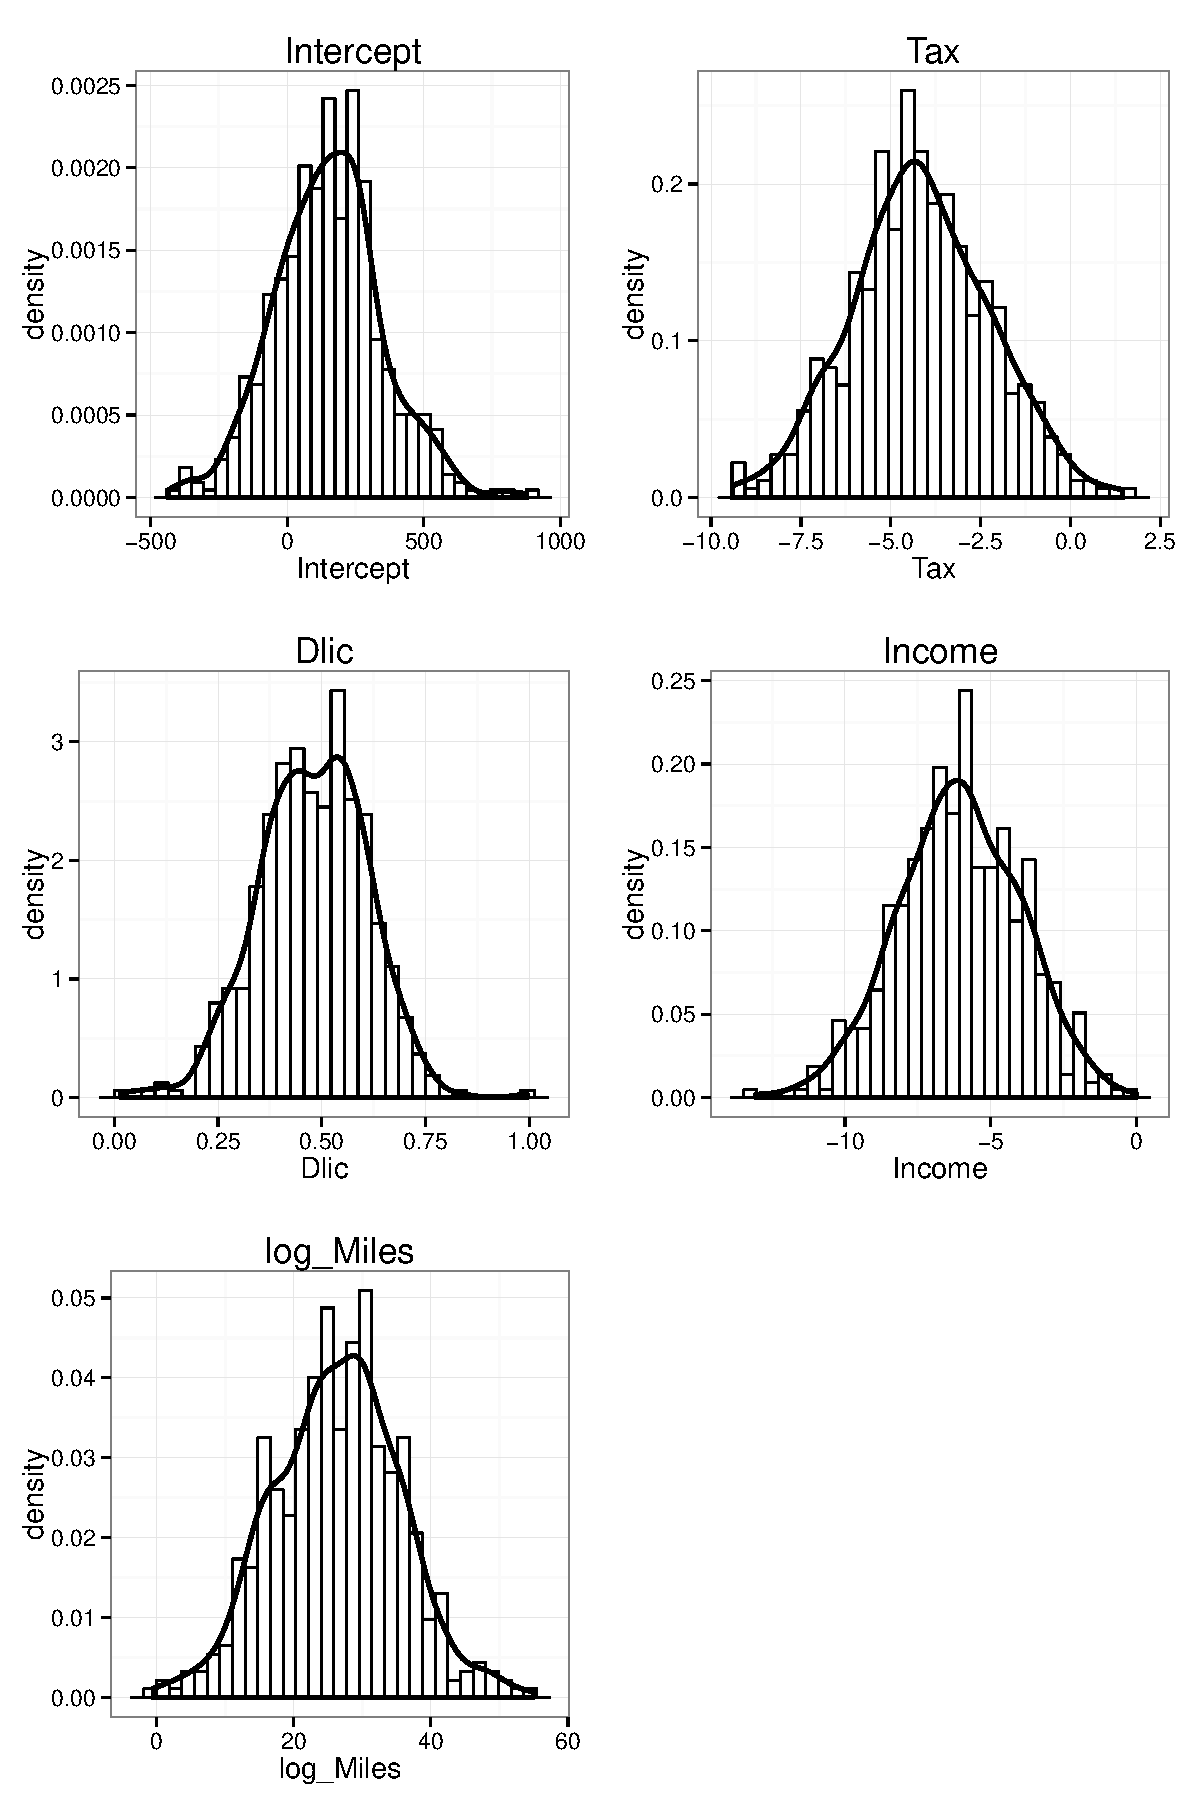
\includegraphics[width=.9\linewidth]{figure/p7102} 

}



\end{knitrout}

According to the histograms above, we can say that the histograms are not all symmetric, and not all of them look like normally distributed data. For example, the coefficient of the intercept seems like skewed, and the distribution of coefficient of \m{Dlic} seems has two peaks, suggesting that they may not be normally distributed, so that the large sample normal theory may not be appropriate to these data. 

However, it's kind of hard to say that the histograms support or refuse the differences between the bootstrap and large sample confidence intervals, because the shape of a histogram is largely affected by the binwitdh we choose, and it's risky to make decision based on histograms. Maybe we need to do some non-parametric test to determine whether they are normally distributed, and then we can say that if the differences are supported.


\end{document}
